\documentclass[a4paper,12pt]{article}
\usepackage[ngerman]{babel}
\usepackage[T1]{fontenc}
\usepackage[utf8]{inputenc}
\usepackage{graphicx}
\usepackage{lmodern}
\usepackage{todonotes}
\usepackage{float}
\usepackage[hyphens]{url} %hyphen for too long urls in the bibiography
\usepackage{listings}
\usepackage[nottoc]{tocbibind} %includes the bibtex bibliography into toc
\usepackage{xcolor} %color instead of color for the definecolor >html<
\usepackage{kpfonts}
\usepackage{natbib}
\usepackage[colorlinks=false]{hyperref}
\usepackage[hang]{footmisc}
\usepackage{fancyhdr}	%package for calling \pagestyle{fancy} 
\usepackage{ifthen} %to set the chaptertitle not in the tocs
\usepackage{titletoc}

\makeatletter
\author{Daniel Sch\"afer} \let\Author\@author
\makeatother

\pagestyle{fancy}
\fancyhf{}
%\fancyhead[RE]{\scshape\nouppercase{\leftmark}}	%LE - left side of the header for even pages, and right side for odd pages
\fancyhead[LO]{\scshape\nouppercase{\rightmark}}
\fancyhead[RO]{\thepage}

\setlength{\textheight}{598pt} %origin 598 in a4
\setlength{\headsep}{20pt}
\setlength{\headheight}{16pt}
\setlength{\topmargin}{0.46cm} %origin a4 = 17pt
\setlength{\marginparwidth}{38pt}
\setlength{\parindent}{0mm}	%neuer paragraph wird nicht eingerückt
\setlength{\parskip}{1mm}	%abstand nach unten hin
\setlength{\skip\footins}{1cm} %before footnote space
\setlength{\footnotemargin}{1em} %standardvalue = 1.8em
\setlength{\intextsep}{20pt plus2pt minus 4pt}	%space between text and the float environment like a picture. 
\setlength{\floatsep}{20pt plus2pt minus 4pt} %two floats behind space between them

\definecolor{graybackgroundColor}{HTML}{E5E5E5} %gray!20 for gray!30 use D9D9D9 for gray!10 F2F2F2

\hypersetup{ %required package hyperrref
  colorlinks   = true, %Colours links instead of ugly boxes
  urlcolor     = blue, %Colour for external hyperlinks
  linkcolor    = black, %Colour of internal links
  citecolor   = black %Colour of citations
}

%with this command its possible to set inline codesnippets with a colorbox
\newcommand{\codeInLine}[1]{%
\colorbox{graybackgroundColor}{\lstinline{#1}} %Colorbox instead of colorbox
}

\lstset{
aboveskip=20pt plus2pt minus 4pt,
belowskip=20pt plus2pt minus 4pt,
	numbers=left,
	numbersep=5pt,
	sensitive=false, %groß kleinschriebung
	tabsize=2,
	backgroundcolor=\color{graybackgroundColor},
	showspaces=false,
  showstringspaces=false,
  showtabs=false,
	breaklines=true, %falls der code über den rand herausragt!
		basicstyle=\footnotesize\ttfamily,
	numberstyle=\tiny\ttfamily,
	captionpos=b,
}

\lstdefinestyle{Cpp} {
language=C++
}
%---------------------------------------------------------------------------------------

\begin{document}

\begin{titlepage}
	\centering
	
\includegraphics[width=0.7\textwidth]{bilder/hskalogo}\par\vspace{1cm}
	\vspace{0.5cm}
	{\Large Studiengang Informatik (Master)}\par
	\vspace{2cm}
	{\huge\bfseries Last-Test von Web-Seiten mit JMeter}\par
	\vspace{2cm}
	{\Large\bfseries Seminararbeit - Ausarbeitung}\par
	\vspace{0.5cm}
	\vspace{3cm}
	
	{\Large Daniel Schäfer (60118)\par}
	\vspace{1cm}
	{\Large\textbf{Betreuer:} Prof.~Dr.~Holger Vogelsang} 
	\vfill
	{\Large Sommersemester 2018\par}
	\vfill
% Bottom of the page
%{\large \today\par}
\end{titlepage}

\pagenumbering{roman}
\setcounter{page}{2}
\thispagestyle{empty} %ohne header und footer
\tableofcontents
\pagebreak
\thispagestyle{empty}
\listoffigures
\pagebreak
%\addcontentsline{toc}{section}{Abbildungsverzeichnis}
%\listoffigures

\pagenumbering{arabic}
\setcounter{page}{5}

\section{Einführung}
Mit dieser Ausarbeitung zur Seminararbeit wird das Performance und Last-Test Programm Apache JMeter ausführlich unter die Lupe genommen. Es werden seine Funktionen und Möglichkeiten erläutert und kurz Alternativen dazu erwähnt. Zusammenfassend werden Vor- und Nachteile aufgelistet, sowie ein Fazit gegeben.

\subsection{Motivation}
Man erlebt es immer wieder, das Webseiten unter zu hoher Last in die Knie gezwungen werden. Sei es nun Amazon, Netflix und Konsorten durch DDoS-Angriffe \cite{online:AmazonDDoS}, oder auch hochschulinterne Seiten, die durch gegebene Anmeldefristen eine hohe Anzahl von gleichzeitigen Benutzern zu bewältigen haben. 

Gerade letzteres Szenario lässt sich im voraus gut vermeiden, da man die grobe Anzahl der Studierenden kennt und somit präventiv die Webseite auf die eingehende Last testen kann. Dabei werden sehr viele nebenläufige Anfragen an einen Anwendung gestartet und die Response Zeiten ausgewertet. Diese Art von Tests nennt man Last oder Performance-Tests und wird in die Klasse der Systemtests kategorisiert \cite{online:LastUndPerformanceTest}. 

Das frei verfügbare, unter Public License Key stehende Java Programm JMeter bietet diese und weitere Funktionalität um die Leistung einer Webseite bis ins kleinste Detail zu analysieren, testen, auswerten und visualisieren.

\subsection{Manuelle vs automatisierte Tests}
Bevor es an das eigentliche Thema JMeter geht, gibt es einen kleinen Exkurs in die sogenannten Systemtests. Diese wurden im vorherigen Abschnitt kurz erwähnt und haben die Besonderheit, dass sie sowohl manuell, als auch automatisiert ausgeführt werden können. 

\subsubsection{Manuelles Testen}
Beim manuellen Testen werden bestimmte Aktionen und Request von mehreren Benutzern nach bestimmten Vorgaben gestartet und die resultierenden Ergebnisse protokolliert. Es liegt auf der Hand, dass diese Art des testens ziemlich zeit -und resourcenaufwändig ist. Zusätzlich muss das Personal, sprich die Tester organisiert, betreut und verpflegt werden. Falls es sich dabei um die Programmierer selbst handelt, stehen diese im Zeitraum auch nicht für andere Tätigkeiten zur Verfügung. Der Faktor Mensch spielt natürlich bei dieser Art der Tests eine Rolle, wodurch nicht ausgeschlossen werden kann, dass Fehler während der Testphasen gemacht und diese entsprechend nicht erfasst werden. \cite[S. 11]{book:ApacheJMeter}

Trotz dieser Nachteile sollte man auf zusätzliche manuelle Tests\footnote{Das sogenannte User Acceptance Testing (UAT) ist gerade im finalen Entwicklungsstadium einer Anwendung unabdingbar. \cite{online:wikiUAT}} einer Anwendung nie verzichten, da eine "`reale"' Person über den Tellerrand schauen kann und es dadurch möglich ist, diverse Bugs ausfindig zu machen, die mit dem eigentlichen Test unter Umständen gar nichts zu tun haben.

\subsubsection{Automatisiertes Testen}
Automatisiertes Testen funktionieren immer dann recht gut, wenn häufige Wiederholungen auftreten. Beispielsweise bei Regressiontests. Aber auch bei Lasttests ist die Testautomatisierung ein gängiges Verfahren. Die Tests laufen in erster Linie mit Software, was zur Folge hat, dass sie ziemlich statisch sind und dadurch beispielsweise keine Ästhetik geprüft werden kann, wie dies etwa bei menschlichen Testpersonen der Fall wäre.

Jedoch haben automatisierte Tests den großen Vorteil, dass sie kosteneffizienter sind. Man benötigt lediglich ein Budget für etwaige Lizenzgebühren der Software oder für den Support. Des weiteren ist man durch Testsoftware in der Lage, sehr viele Benutzer gleichzeitig zu erzeugen und parallel auf ein System zugreifen zu lassen. Mit Testskripten sogar rund um die Uhr \cite{online:Testautomatisierung}. Dadurch werden Systeme bis zur ihren Grenzen und darüber hinaus getestet.

\section{Apache JMeter}
Wen man sich nun für die Testautomation entschieden hat, steht man vor der Wahl einer entsprechenden Software. Diese befinden sich in einer Preisspanne von kostenlos bis hin zu einem fünfstelligen Bereich. Die Wahl hängt letzten Endes von den eigenen Anforderungen ab \cite[S. 15]{book:ApacheJMeter}. Da sich die Arbeit auf JMeter bezieht richten wir unser Augenmerk auf diese spezielle Software.

Wie man in Abbildung~\ref{fig:jmeter_gui} erkennen kann, erscheint Apache JMeter mit seinen "`Metal-Look-and-Feel"' \cite{online:wikiSwing} Widgets wie das Relikt aus einer längst vergangenen Zeit. Man sollte sich jedoch von der veralteten und trägen Swing-basierten GUI nicht täuschen lassen, denn hinter der Oberfläche steckt ein mächtiges Werkzeug, mit dem man alle möglichen Arten von Tests erstellen und ausführen kann. \cite{online:heiseJMeterOderGatling}

Tatsächlich stammt JMeter aus einer Zeit als das Web und Application Server noch in den Kinderschuhen steckten. Ursprünglich wurde es entwickelt um den Application Server Tomcat zu testen. Seitdem wurde das Programm fortlaufend weiter entwickelt, so dass man heute in der Lage ist diverse Tests zu realisieren. Von verteilten Tests in der Cloud, über das Testen von dynamischen Webseiten bis hin zu Javas JUnit Tests. \cite{online:ApacheJMeter}

\begin{figure}[htb]%[ht]
 \centering
    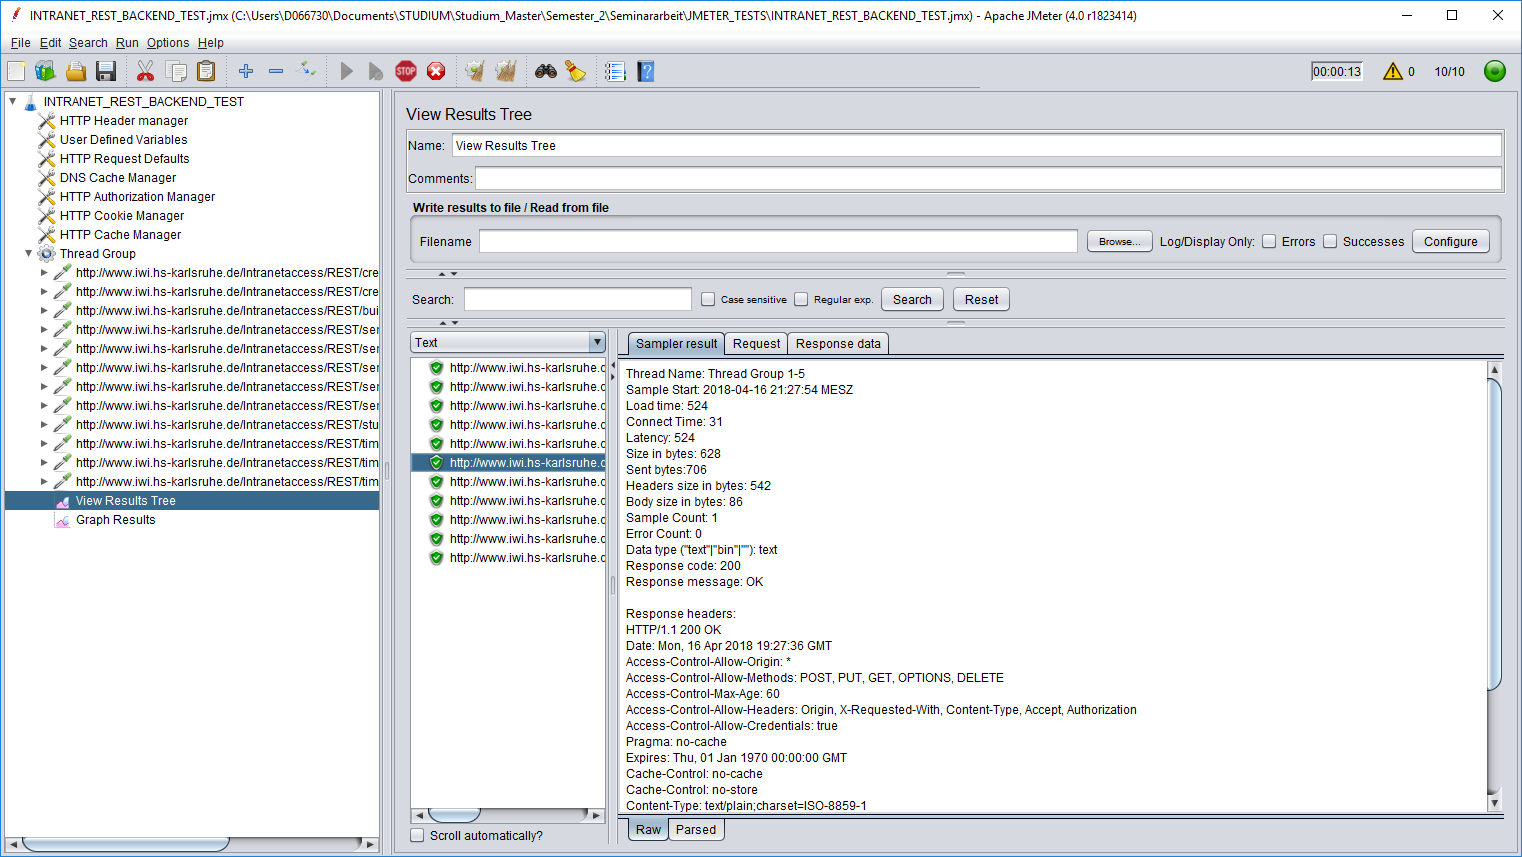
\includegraphics[width=1\textwidth]{bilder/jmeter_1.png}
  \caption{Apache JMeter GUI}
  \label{fig:jmeter_gui}
\end{figure}
Apache JMeter wurde in Java geschrieben und kann durch seine platformunabhängigkeit unter jedem beliebigen Betriebssystem, welches eine Java Runtime Environment (JRE) installiert hat, verwendet werden. Neben der GUI kann man Apache JMeter auch mit der Kommandozeile bedienen. Dies ist gerade bei speicherintensiven Lasttests empfehlenswert, da die GUI schnell an ihre Grenzen kommt und sich die Testergebnisse nicht mehr genau erfassen lassen. Mehr zum Thema Kommandozeile in Abschnitt~\ref{chap:jmeter_commandline}.

Apache JMeter bietet zusätzlich eine gut dokumentierte API an, mit der es möglich ist das Programm selbständig zu erweitern.

\subsection{Historisches}
Ursprünglich wurde Apache JMeter von Stefano Mazzocchi, seiner Zeit Entwickler bei der Apache Software Foundation, programmiert um die Performance von Apache Tomcat (damals noch Apache JServ) zu testen. Kurz danach wurde das Programm neu entworfen und mit einer verbesserten GUI und zusätzlichen Möglichkeiten von Funktionstests ausgestattet. Im Jahr 2011 wurde JMeter zu einem sogenannten Top Level Apache project, was eine offizielle Homepage und ein Projekt Management Committee mit sich brachte \cite{online:officialJMeter}.

Mittlerweile ist Apache JMeter ein wichtiger Bestandteil von Performance Tests in sehr vielen Firmen geworden. Großkonzerne wie SAP oder 1\&1 verwenden regelmäßig JMeter um die Verfügbarkeit ihrer Produkte unter hoher Last zu prüfen. 

\subsection{Was kann JMeter}
Apache JMeter dient in einer Client/Server Landschaft als Client und kann dadurch Anfragen an bestimmte Anwendungen absetzen. Dadurch erhält man unter anderem die Responsezeit, Responsemesage oder aber auch den Speicherverbrauch.

Anfragen können sowohl an statische als auch an dynamische Resourcen erfolgen. Darunter fallen unter anderem statische Dateien, Servlets, FTP Server, Datenbanken, Java Objekte und Skripte.
Um diese Anfragen in einer entsprechend großen Anzahl abzufeuern, bietet das Programm die Simulation von vielen gleichzeitigen Benutzern an. Diese Threads lassen sich in einzelne Thread Gruppen unterteilen.

In JMeter ist es ebenfalls möglich, den Test in eine Cloud Infrastruktur auszulagern und die Tests unabhängig vom eigenen System bzw. Hardware laufen zu lassen. \todo{hier noch entsprechendes Chapter und besser formulieren} Es ist auch möglich die Testfälle in ein verteiltes System zu packen und dadurch deutlich mehr Resourcen zu verwenden. \todo{Cloud + Verteilte Systeme noch recherchieren}

Nach den Tests bietet JMeter ein HTML Dashboard an, in dem sehr viele Informationen über die Anfragen und Ergebnisse in Tabellen und Statistiken grafisch aufbereitet dargestellt werden. Abbildung~\ref{fig:dashboard} zeigt einen Ausschnitt des Dashboards, welches im Abschnitt~\ref{chap:html_dashboard} genauer untersucht wird.  

\begin{figure}[htb]%[ht]
 \centering
    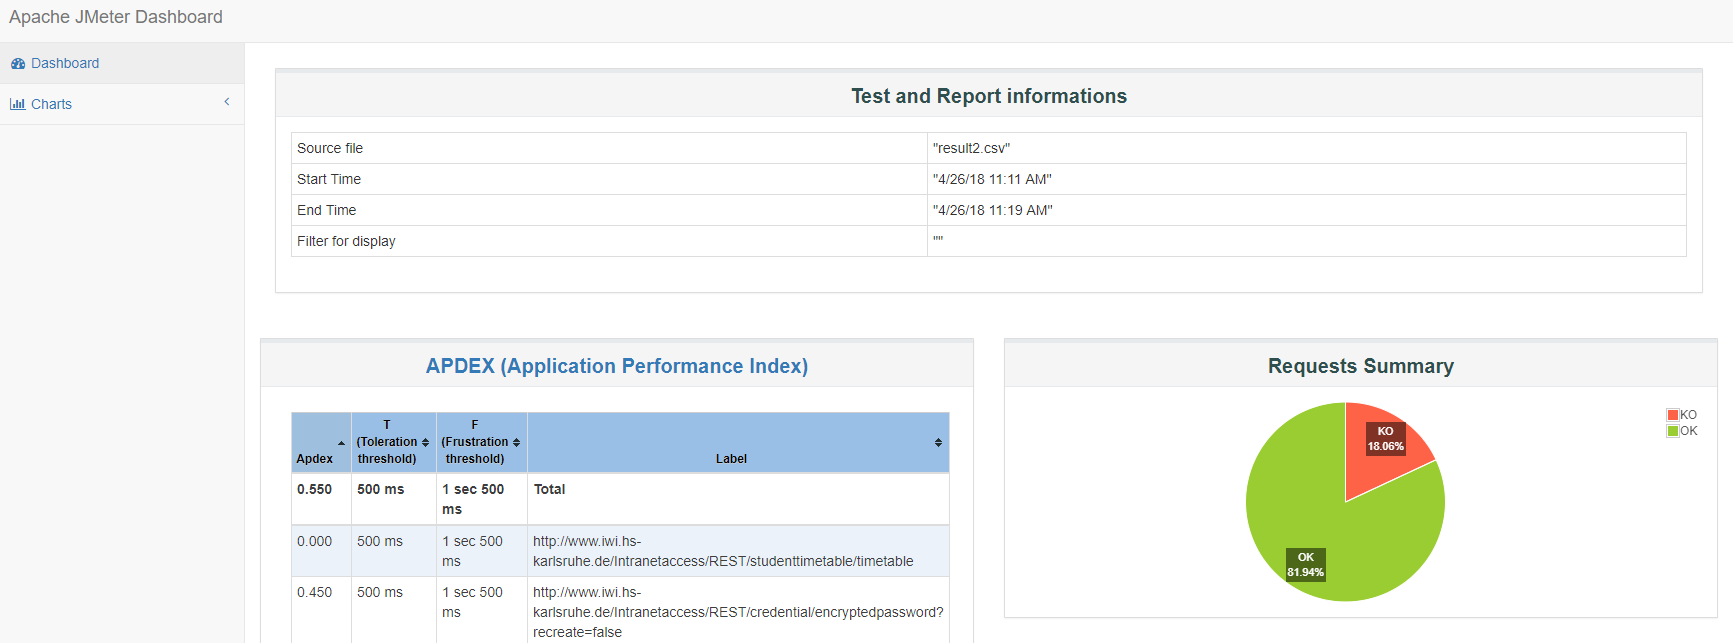
\includegraphics[width=1\textwidth]{bilder/dashboard.png}
  \caption{HTML Dashboard Report}
  \label{fig:dashboard}
\end{figure}

Eine weitere nützliche Funktion ist das Aufzeichnen von Userinteraktionen. Dieser Http Test Script Recorder wird in JMeter mit bestimmten Filtern und Pattern vorkonfiguriert und gestartet. Jede Aktion im Browser mit der entsprechenden URL und Port wird dann als einzelner HTTP Request Sampler angelegt. Der Recorder wird initial einmal ausgeführt und kann dann für diverse Tests recycelt werden.    

Seit der JMeter Version 2.1.2 ist es außerdem möglich in Java geschriebene JUnit Tests als JUnit Sampler zu importieren und ausführen. Diese nützliche Funktion wird im Abschnitt \nameref{chap:junit_tests} untersucht.

\subsection{Installation}
Im folgenden Kapitel werden notwendige Schritte zur Inbetriebnahme von Apache JMeter erklärt.

\subsubsection{Einrichten der Umgebung}
Apache JMeter wurde als reine Java Anwendung entwickelt. Sie ist dadurch platformunabhängig und benötigt keine zusätzlichen Treiber oder Installation. Alle notwendigen Abhängigkeiten und Klassen sind im entsprechenden Archiv hinterlegt. Zum Starten muss man lediglich die *.jar Datei aus dem Verzeichnis ausführen.

Auf der offiziellen Seite von Apache JMeter \url{http://jmeter.apache.org/download_jmeter.cgi} muss man sich zunächst eine Release Version herunterladen. Den Build entpackt man dann in ein beliebiges Verzeichnis, beispielsweise \codeInLine{C:\\\\Program Files\\jmeter\\}.
Es sollte bereits eine aktuelle JRE vorhanden sein, da diese Grundvorausstzung ist um *.jar Dateien auszuführen. Prüfen kann man dies, indem man in der Kommandozeile den Befehl \codeInLine{java -version} eingibt. Wenn keine JRE installiert ist kommt eine entsprechende Meldung, dass der Befehl nicht gefunden wurde. In diesem Fall hilft eine Installation der Java runtime environment von der offiziellen Oracle Seite unter \url{http://www.oracle.com/technetwork/java/javase/downloads/index.html}.

Im Installationspfad befinden sich mehrere Unterverzeichnisse. Wichtig sind hier der \codeInLine{\\bin} Ordner und der \codeInLine{\\lib} Ordner. Im ersteren befindet sich die ApacheJMeter.jar Datei welche die GUI von JMeter startet. Im lib Verzeichnis sind alle Libraries und Erweiterungen hinterlegt. Dies ist auch der Ort an dem zusätzliche Third-Party -Plugins hineinkopiert werden müssen.

\subsubsection{Starten von JMeter}
JMeter lässt sich wie bereits erwähnt als GUI bzw. als Kommandozeilenprogramm verwenden.  Um JMeter als GUI zu starten kann man direkt die ApacheJMeter.jar ausführen. Sitzt man hinter einer Firewall empfiehlt es sich die GUI via Kommandozeile zu starten. Folgende Parameter  sollten dabei verwendet werden:

\begin{table}[H]
	\centering
	\begin{tabular}{|l|l|}
		\hline
		\textbf{Parametername} & \textbf{Bedeutung} \\
		\hline
		-H & Proxy Server Hostname bzw. IP-Adresse \\
		-P & Port vom Proxy Server \\
		-N & Host ohne Proxy (localhost) \\ 
		-u & Benutzername für den Proxy \\
		-p & Passwort für den Proxy \\
		\hline
	\end{tabular}
	\caption[tab_parameter_gui]{Befehle für Firewall Einstellungen}
	\label{tab_parameter_gui}
\end{table}

Beispiel: Aus der Kommandozeile ins /bin Verzeichnis von JMeter navigieren und folgenden Befehl ausführen: 
\begin{lstlisting}
jmeter -H 196.168.178.1 -P 1337 -u lindan -a hispassword -N localhost
\end{lstlisting}
Alternativ dazu die Befehle der JMeter Kommandozeile ohne GUI:

\begin{table}[H]
	\centering
	\begin{tabular}{|l|l|}
		\hline
		\textbf{Parametername} & \textbf{Bedeutung} \\
		\hline
		-n & non-GUI - keine GUI Oberfläche \\
		-t & jmx Datei, dass die Testfälle enthält \\
		-l & jtl Datei, in dem die Logs gespeichert werden \\ 
		-r & Verwende alle Remote Server aus jmeter.properties \\
		\hline
	\end{tabular}
	\caption[tab_parameter_non_gui]{Befehle für JMeter Kommandozeile}
	\label{tab_parameter_non_gui}
\end{table}

Beispiel um die test.jmx Datei auszuführen und in logtest.jmx zu speichern: Aus der Kommandozeile ins /bin Verzeichnis von JMeter navigieren und folgenden Befehl ausführen: \
\begin{lstlisting}
jmeter -n -t test.jmx -l logtest.jtl
\end{lstlisting}
Mehr zum Thema GUI und Kommandozeilenaufurf in den nachfolgenden Kapiteln.

\subsection{JMeter GUI}
Die GUI von JMeter ist die erste Anlaufstelle für Anfänger und interessierte Benutzer. Hier kann man schnell und einfach Testaufrufe erzeugen und Ergebnisse anhand von Graphen und Tabellen anzeigen. 

Die GUI wird von erfahrenen Anwendern hauptsächlich dazu verwendet um die Test Sampler zu generieren, die dann später aus der Kommandozeile heraus als *.jmx Dateien gestartet werden.

Hier kann man auch den HTTP Test Script Recorder konfigurieren und starten, mit dem es möglich ist, diverse HTTP Anfragen an Webseiten aufzuzeichnen. Mehr zum Thema Recording und Aufzeichnen von Aktionen in Kapitel \ref{sec:wissenswertes}. Abbildung \ref{fig:gui_graph} zeigt die GUI beim Abarbeiten mehrerer gleichzeitiger Anfragen an eine Webseite. Der Graph kann das ganze zusätzlich visualisieren. Dadurch erkennt man, an welchen Stellen noch  optimiert werden kann.

\begin{figure}[htb]%[ht]
 \centering
    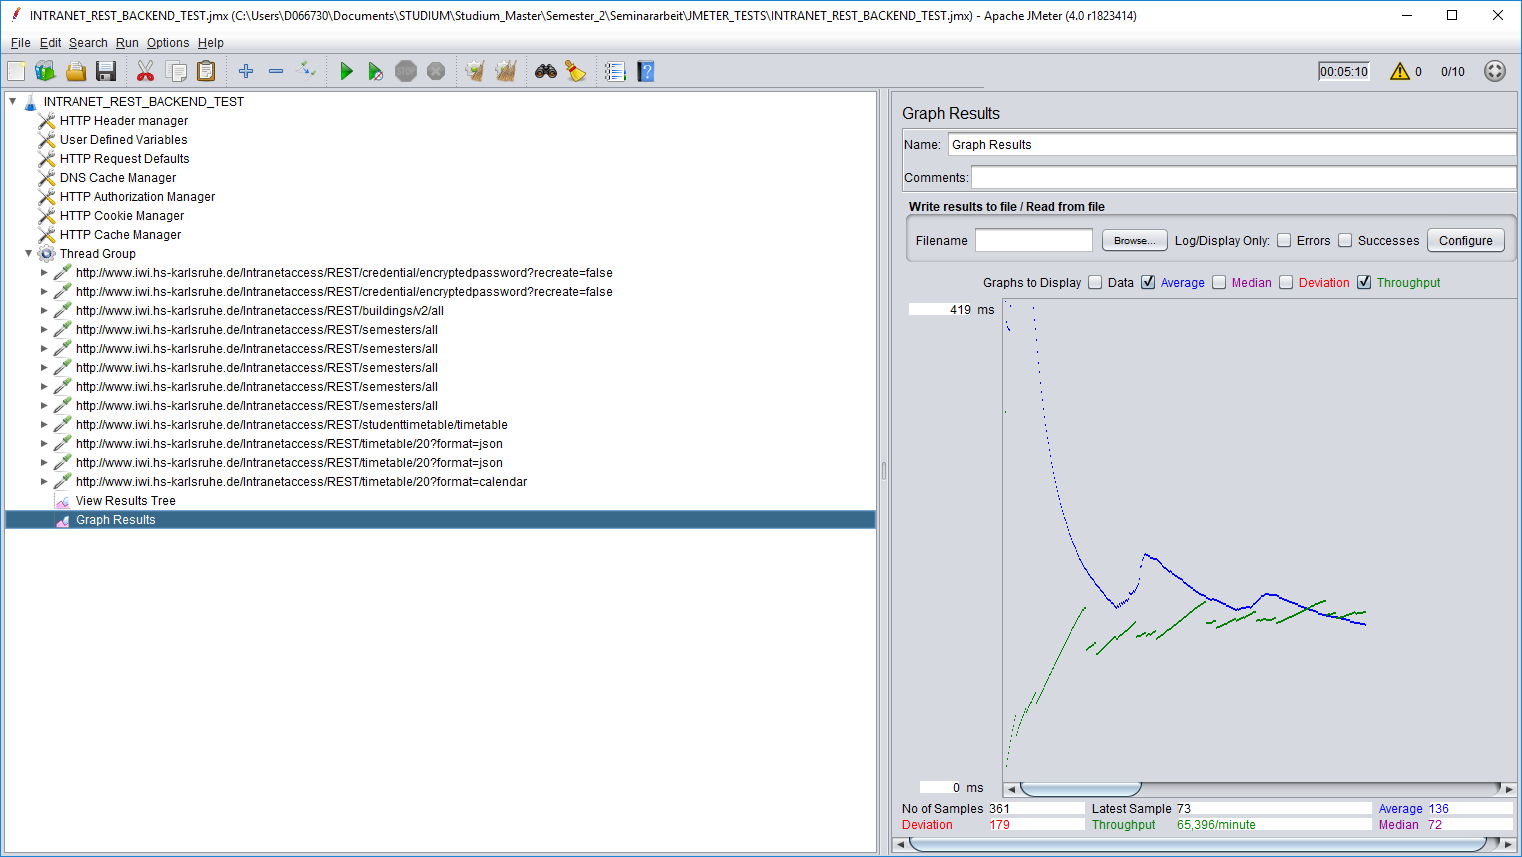
\includegraphics[width=1\textwidth]{bilder/jmeter_2.png}
  \caption{JMeter GUI mit Graph}
  \label{fig:gui_graph}
\end{figure}

\subsection{JMeter Kommandozeile}
\label{chap:jmeter_commandline}
Möchte man nun einen auswendigeren Lasttest machen, eignet sich die GUI ab einer gewissen Anzahl von gleichzeitigen Benutzern nicht mehr. Durch die steigende Anzahl der Anfragen wird auch der Resourcenbedarf immer größer und der ohnehin schon recht hohe Speicherbedarf der GUI selbst kann sich dann negativ auf die Messergebnisse auswirken und diese verfälschen.

Hier kommt der sogenannte "`Non-GUI Modus"' ins Spiel. Dies ist die Bezeichnung um JMeter in der Kommandozeile auszuführen. Mit Hilfe des Kommandozeilenaufrufes lassen sich am Ende des Tests CSV oder XML Dateien erstellen, die Testergebnisse beinhalten. Auch der HTML Dashboard Report lässt sich nur hier generieren.

\subsubsection{Ausführen des Non-GUI Modus}
Zuerst sollte ein Testscript verfügbar sein. In diesem sind alle Requests und Konfigurationen wie Cache/Cookie verhalten und Authorization Management enthalten. Man kann hier ein vorhandenes File verwenden oder in JMeter selbst ein neues jmx-File erzeugen. Minimale Voraussetzungen sind eine Thread Group sowie ein Sampler, beispielsweise ein HTTP Request, mit entsprechender URI und Operation.

Nun startet man die Kommandozeile und navigiert in das /bin Verzeichnis von JMeter. Dort startet man den Test via folgendem Befehl:
\begin{lstlisting}
jmeter -n -t [Pfad zum jmx-file] -l [Pfad zum result file] -e -o [Pfad zum HTML Dashboard Ordner]
\end{lstlisting} 
In der folgenden Tabelle sieht man einige häufig verwendete Parameter und ihre Bedeutung. Um eine Übersicht aller Parameter zu erhalten, kann man in der Kommandozeile den Befehl \codeInLine{jmeter -?} ausführen. Ein zweiter sehr nützlicher Befehl ist \codeInLine{jmeter -h}, welcher eine Vorauswahl von Kommandozeilenbefehle von JMeter anbietet.
\begin{table}[H]
	\centering
	\begin{tabular}{|l|l|}
		\hline
		\textbf{Parametername} & \textbf{Bedeutung} \\
		\hline
		-n & Non-GUI Modus \\
		-t & Pfad zum JMeter Skript; in Verbindung mit -n \\
		-l & Pfad zum Result File \\
		-? & Hilfe; zeigt alle Parameter an \\
		-h & Beispielbefehle, die man verwenden kann \\
		-L & Log level - Wann soll etwas geloggt werden \\
		-e & Um HTML Reports zu erzeugen\\
		-o & Pfad zum Output Folder; in Verbindung mit -e or -g \\
		-g & HTML Report wird aus einem CSV file erzeugt \\ 
		\hline
	\end{tabular}
	\caption[tab_parameter_non_gui]{Befehle der JMeter Kommandozeile}
	\label{tab_parameter_non_gui}
\end{table}

Pauschal kann man sagen, dass man die GUI bei kleineren Tests bzw. Testplanerstellung verwendet. Für alles andere sollte der Non-GUI Modus die erste Wahl sein.

\section{Der Testplan}
Nach dem ganzen Vorgeplänkel geht es nun an die Erstellung eines ersten Testplans für JMeter.
Doch was ist überhaupt ein Testplan? Jeder JMeter Test hat genau einen Testplan, der als Wurzel in der Hierarchie angelegt ist. Man kann ihn sich als einen Container vorstellen, der weitere Komponenten beinhaltet kann, die nötig sind um einen Testlauf erfolgreich zu starten. Der Testplan ist ein Skript in einem speziellen JMX Format. Betrachtet man die Datei in einem Texteditor erkennt man, dass es sich hier um eine xml-Datei handelt (Siehe Abbildung \ref{fig:jmx_xml}). Nach anlegen und abspeichern des Testplans kann man diesen via Kommandozeile oder GUI starten. Falls man auf einem Testplan die Option "`Functional Test Mode"' aktiviert, sorgt das dafür, dass JMeter den Response jedes Sample-Aufrufs in ein Log-File speichert. Diese Log-Files lassen sich in den Listenern konfigurieren.

\begin{figure}[htb]%[ht]
 \centering
    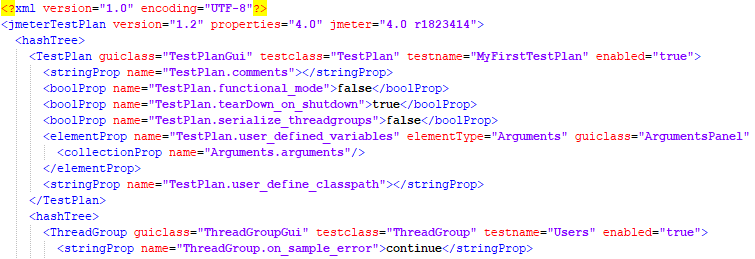
\includegraphics[width=1\textwidth]{bilder/jmx_xml.png}
  \caption{JMX-Datei in Notepad++ geöffnet}
  \label{fig:jmx_xml}
\end{figure}

\subsection{Elemente eines Testplans}
Um einen Test zu starten benötigt man mindestens einen Testplan, darunter eine Thread Group sowie einer oder mehrere Sampler. Nachfolgend eine Auflistung der wichtigsten Elemente und ihre Funktion, die in einem Testplan verwendet werden.

\subsubsection{Thread-Groups}
Zu jedem Testplan gehört mindestens eine Thread-Group. Diese steht stellvertretend für die Anzahl der gleichzeitigen Benutzer und Wiederholungen, die simuliert werden. Abbildung~\ref{fig:thread_group} zeigt die wichtigsten Einstellungen der Thread Group. Neben den selbsterklärenden Bezeichnungen und Werte gibt es noch die Ramp-Up Period. Diese gibt an, in welcher Zeitspanne die Threads erzeugt werden sollen.
Angenommen man gibt 10 Threads an und die Ramp-Up Period stellt man auf 20 Sekunden, wird alle 2 Sekunden ein neuer Thread erzeugt. Dies verhindert ein gleichzeitiges Erzeugen aller Threads und dadurch eine zu hohe Systemauslastung zu Beginn des Tests.

\begin{figure}[htb]%[ht]
 \centering
    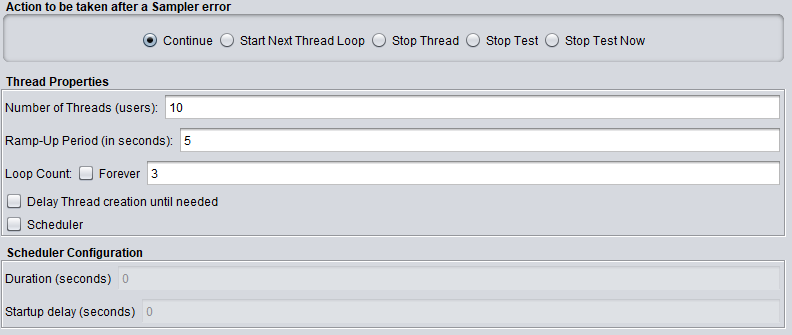
\includegraphics[width=1\textwidth]{bilder/thread_group.png}
  \caption{Wichtige Einstellungen der Thread-Group}
  \label{fig:thread_group}
\end{figure}

Thread-Groups kann man zusätzlich auch als setUp- oder tearDown-Gruppen anlegen. Diese werden analog zu JUnit Tests entsprechend vor der eigentlichen Thread-Group gestartet oder eben nach Beendigung aller Thread-Groups. Sehr hilfreich, wenn man beispielsweise Werte aus einer Datenbank auslesen und diese in Variablen speichern möchte, bevor der eigentliche Test beginnt und das Auslesen nicht in den eigentlichen Test mit einfließen sollen \cite{online:testingJournals}.

\subsubsection{Sampler}
Sampler und Logic Controller steuern die Abarbeitung eines Tests. Dabei sind Sampler für das Senden eines Requests verantwortlich und die Logic Controller für den zeitlichen Aspekt, also wann dieser Request gesendet wird. Innerhalb der Thread-Group lassen sich mehrere Sampler anlegen. Diese Sampler sind die eigentlichen Anfragen des Tests und stellen die Verbindung zu den zu testenden Objekten her. Es gibt Sampler für die unterschiedlichsten Protokolle wie HTTP, FTP, JDBC SOAP/XML und Java-Objekte. 

HTTP-Sampler sind die wohl am häufigsten eingesetzten Sampler. Mit ihnen lassen sich unter anderem REST Aufrufe an entsprechende Server starten. Abbildung \ref{fig:http_request_sampler} zeigt einen HTTP-Request Sampler an die hochschulinterne API mit der GET-Methode.

\begin{figure}[htb]%[ht]
 \centering
    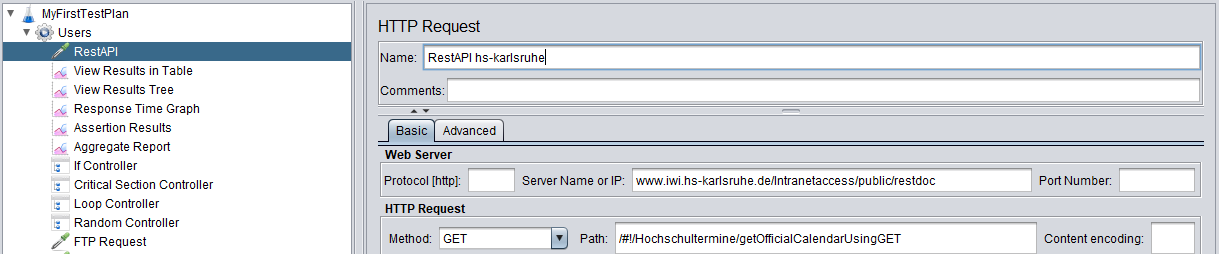
\includegraphics[width=1\textwidth]{bilder/http_request_sampler.png}
  \caption{HTTP-Request Sampler}
  \label{fig:http_request_sampler}
\end{figure}

\subsubsection{Logic Controller}
Der Logic Controller steuert den zeitlichen Ablauf einzelner Teile, insbesondere der Sampler und kann man unter anderem angeben, wie oft ein Sampler wiederholt werden soll oder wann dieser gestartet werden soll. Aber auch komplexere Szenarien, etwa durch reguläre Ausdrücke bei beim If-Controller sind machbar.

\subsubsection{Timer}
Durch einen Timer kann man eine Verzögerung nach jedem Thread einbauen, so dass der Test für kurze Zeit angehalten wird. Es gibt konstante und Zufallstimer.

\subsubsection{Config Elements}
Zu einzelnen Samplern oder Thread-Groups gibt es noch diverse Config Elements. Diese dienen dazu default parameter einmalig anzulegen und darauf zuzugreifen. Wird dann in den jeweiligen Controllern kein Wert in die entsprechenden Label eingetragen, wird auf den Wert im Config Element zurückgegriffen. Speziell für HTTP-Sampler gibt es darüber hinaus noch weitere Config Elemente, wie Header, Authorization oder Cookie Informationen, die man zentral für den ganzen Testplan abspeichern kann \cite{online:performanceTools}.

\subsubsection{Listener}
Listener sind Elemente die Informationen über die Ergebnisse der Performance Tests enthalten. Es gib verschiedene Arten von Listenern, wie etwa den Graph Result Listener, den View Results Tree Listener oder den Aggregation Report. Wichtiger Hinweis an der Stelle: Egal welcher Listener verwendet wird, die Daten die gespeichert werden sind immer die selben. Lediglich die Darstellung dieser auf dem Ausgabemedium unterscheidet sich. Man kann Listener an jede beliebige Stelle im Test hängen; auch unter einem Testplan. Es werden jedesmal die Daten gesammelt, die ab der eingehängter Stelle präsent sind.

\subsubsection{Pre Processors}
modify the request
\subsubsection{Post processor}
parse the response

\subsubsection{Assertions}
Mit JMeter lassen sich auch Assertions untersuchen. Dazu wird der Response eines Requests auf seinen Statuscode hin überprüft. Auch Antwortzeiten lassen sich mit Hilfe von Assertions prüfen. Liegt die Response in einer bestimmten Zeitspanne oder überschreitet der Response diese Zeit kann man entsprechend darauf reagieren.  

\section{Aufzeichnen von Aktionen}
Es leuchtet ein, dass wenn man eine Webseite auf ihre Performance untersuchen will, sehr viele, möglichst unterschiedliche Anfragen an die Seite stellen möchte. Es soll natürlich eine Testabdeckung von nahezu 100\% erreicht werden und so gut es geht alle Pfade innerhalb der URL zumindest einmal besucht werden. Um in JMeter nicht jeden Sampler einzeln anzulegen, gibt es diverse Tools, die Aktionen auf Webseiten aufzeichnen, die in den folgenden Kapiteln kurz erwähnt werden.  

\subsection{Chrome Plugin Blazemeter}
Ein wohl recht bekanntes Tool ist Blazemeter. Das kostenlose platformunabhängige Chrome-Plugin ist in der Lage Aktionen von bestimmten URLS aufzunehmen und danach zu exportieren. Ein kleiner Wermutstropfen muss man hier noch zu erwähnen. Für das exportieren der Aufzeichnung in das JMX Format muss man sich für die Anwendung kostenlos registrieren. Wem dies nichts ausmacht, erhält mit Blazemeter ein solides Recorcing Tool, dass eng mit JMeter zusammenarbeitet. 

\begin{figure}[htb]%[ht]
 \centering
    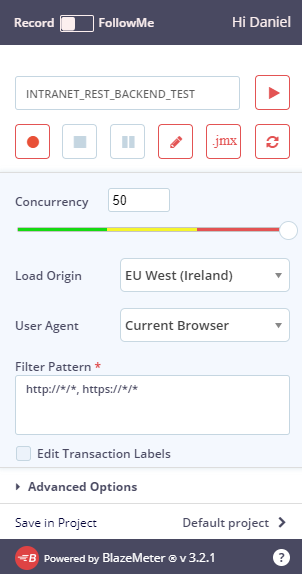
\includegraphics[width=0.2\textwidth]{bilder/blazemeter.png}
  \caption{Blazemeter}
  \label{fig:blazemeter}
\end{figure}

\subsection{Spezielle Software}
Natürlich gibt es auch die Möglichkeit speziell für Recording entwickelte Software zu verwenden. Diese gibt es in Hülle und Fülle im Internet. Sowohl kostenpflichtig als auch Open-Source-Lösungen. Für Windows Nutzer gibt es beispielsweise die Software BadBoy. Unter \url{http://www.badboy.com.au} kann man sich die neuste Version unter Angaben eines Namen und Email Adresse herunterladen und installieren. Abbildung~\ref{fig:badboy} zeigt die Oberfläche von BadBoy in Aktion. 

\begin{figure}[htb]%[ht]
 \centering
    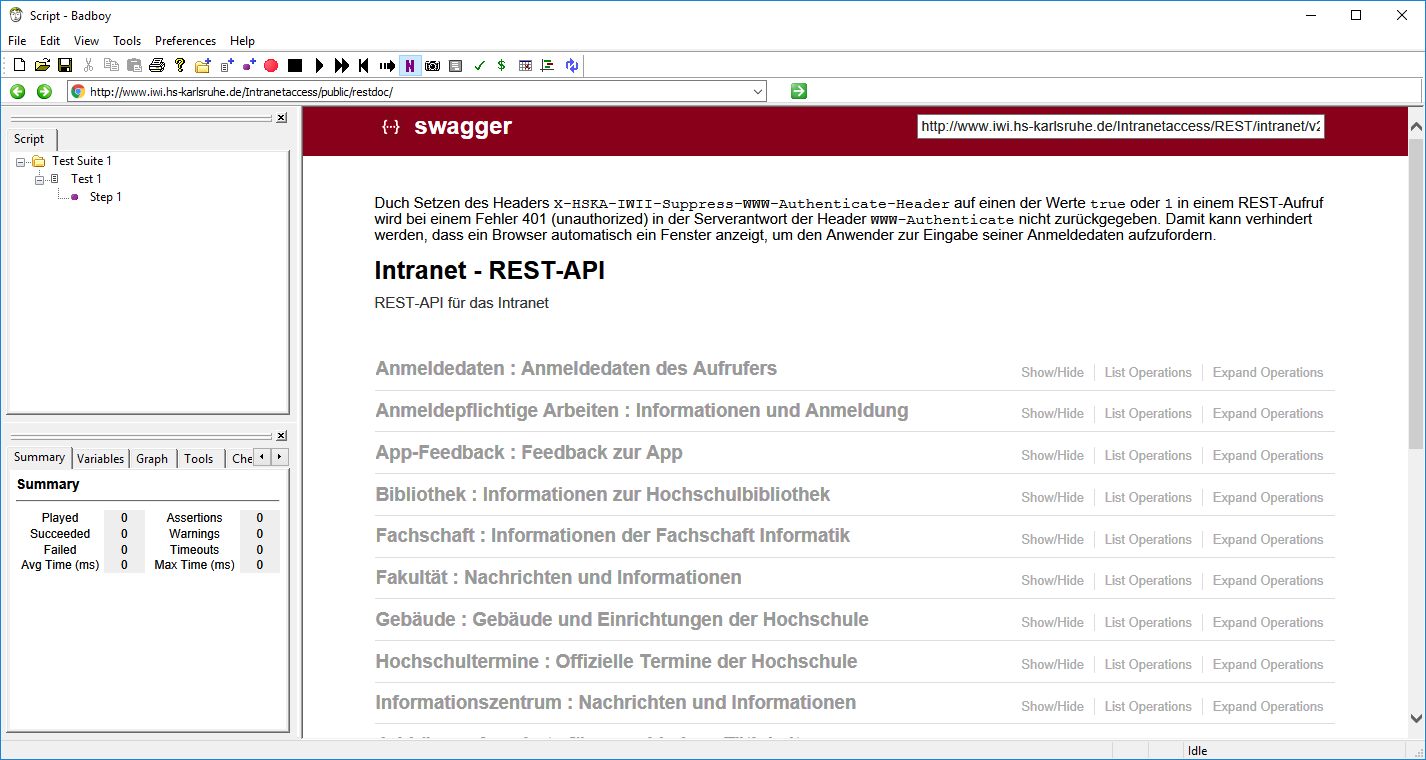
\includegraphics[width=1\textwidth]{bilder/badboy.png}
  \caption{BadBoy Recording Software}
  \label{fig:badboy}
\end{figure}

\subsection{Build-in Lösung}
Für JMeter Enthusiasten gibt es einen integrierten Testscript Recorder. Diesen findet man entweder beim Testplan unter folgendem Menüpunkt \codeInLine{Add -> Non-Test-Elements\n -> HTTP Test Script Recorder} oder über den Weg \codeInLine{File -> Templates... -> Recording Template Create}.
Abbildung~\ref{fig:https_recorder} zeigt den erstellten Recorder. Nachdem der Port angepasst wurde klickt man auf Start und muss nun im Browser den entsprechenden ProxyServer konfigurieren. Als Adresse wählt man \codeInLine{localhost} und der Port entsprechend den JMeter Settings. Jede Aktion die nun im Browser getriggert wird, wird als Sampler im JMeter Testplan unter der entsprechenden Thread-Group angelegt. Zusätzliche Cookies und Variable Konfigurationen werden automatisch angelegt.

\begin{figure}[htb]%[ht]
 \centering
    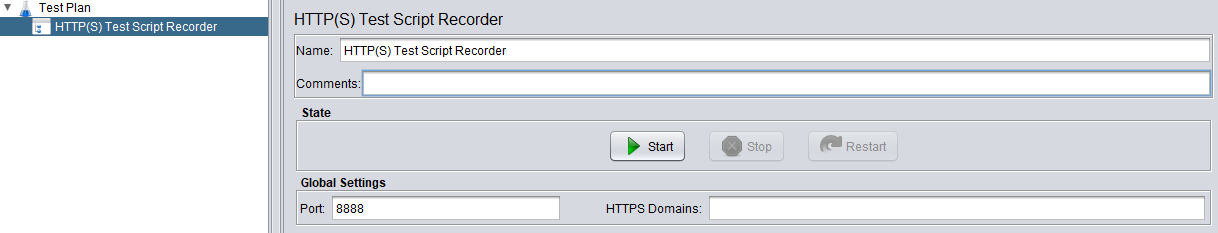
\includegraphics[width=1\textwidth]{bilder/https_recorder.png}
  \caption{HTTP Test Script Recorder}
  \label{fig:https_recorder}
\end{figure}

\section{Lasttests von Webseiten}

\section{Funktionale Tests}

\section{JUnit Tests}
\label{chap:junit_tests}

\section{Auswertung HTML Dashboard}
\label{chap:html_dashboard}
APDEX index. selbst bearbeiten in /bin/user.properties file.

\section{Wissenswertes und Besonderheiten}
\label{sec:wissenswertes}
Man kann die Ergebnisse zur Laufzeit in Logfiles schreiben.

\subsection{JMeter Plugin Manager}

\subsection{Datenbankabfragen - Datenbank testplan?}
Auch datenbankabfragen lassen sich damit visualisieren

Falls interersse besteht, wie es funktioniert bitte in die Ausarbeitung schauen.
Thread Gruppe erstellen -> Configuration (JDBC Connection Configuration)
MySQL jdbc jar in lib folder von jmeter adden 
DAnn Sampler -> JDBC Request and put in values.. z.b. select * from table


\subsection{Virtuelle Compute Unit}
In die Cloud um an einer zentralen stelle viele rechner zu bedienen?
Eventuell viele Rechner simulierenö

\subsection{JMeter change Settings}
In /bin folder von JMeter kann man die Datei user.properties öffnen und Werte anpassen.

\section{Nachteile von JMeter}
Wenn ein Variablenfeld required ist. z.b. bei JDBC Connection Configuration. dann wird einem der fehler nicht direkt im feld angezeigt.

Ziemlich resourcenhungrig. Trotz 16GB Arbeitsspeicher hängt sich das Ding gerne mal auf.

Passwort im Klartext. Gerade wenn man das zeug verteilt verwendet mit mehreren benutzern nicht sehr sicher

Keine Captcha erkennung
\section{Alternativen}
\subsection{Gatling}
https://www.heise.de/developer/artikel/Last-und-Performance-Tests-mit-JMeter-oder-Gatling-3648505.html
\subsection{Selenium}

\section{Fazit}
Alles in allem ist JMeter ein Super tool

\pagebreak
\thispagestyle{empty}
\bibliographystyle{plain}
\bibliography{Bibliography}

\end{document}